\documentclass[11pt]{beamer}
\usetheme[
%%% options passed to the outer theme
    progressstyle=fixedCircCnt,   %either fixedCircCnt, movCircCnt, or corner
    rotationcw,          % change the rotation direction from counter-clockwise to clockwise
    shownavsym          % show the navigation symbols
  ]{AAUsimple}

\definecolor{darkblue}{RGB}{51,51,179}

% If you want to change the colors of the various elements in the theme, edit and uncomment the following lines
% Change the bar and sidebar colors:
\setbeamercolor{AAUsimple}{fg=gray!50 ,bg=darkblue}
\setbeamercolor{sidebar}{bg=gray!20}
\setbeamercolor{frametitle}{fg=darkblue!5,bg=darkblue}
% Change the color of the structural elements:
\setbeamercolor{structure}{fg=darkblue}
% Change the frame title text color:
%\setbeamercolor{frametitle}{fg=darkblue!20}
% Change the normal text color background:
%\setbeamercolor{normal text}{fg=black,bg=gray!10}
% ... and you can of course change a lot more - see the beamer user manual.

\usepackage[utf8]{inputenc}
\usepackage[spanish]{babel}
\usepackage[T1]{fontenc}
% Or whatever. Note that the encoding and the font should match. If T1
% does not look nice, try deleting the line with the fontenc.
\usepackage{helvet}

% colored hyperlinks
\newcommand{\chref}[2]{%
  \href{#1}{{\usebeamercolor[bg]{AAUsimple}#2}}%
}

\title{Control de acuarios con la CIAA}

\subtitle{Presentación del Trabajo Final}  % could also be a conference name

\date{\today}

\author{ Ing. Patricio Bos }

% - Give the names in the same order as they appear in the paper.
% - Use the \inst{?} command only if the authors have different
%   affiliation. See the beamer manual for an example

\institute[
%  {\includegraphics[scale=0.2]{aau_segl}}\\ %insert a company, department or university logo
  Dept.\ de electrónica\\
  Facultad de Ingeniería\\
  Universidad de Buenos Aires
] % optional - is placed in the bottom of the sidebar on every slide
{% is placed on the bottom of the title page
  Carrera de Especialización en Sistemas Embebidos\\
  Facultad de Ingeniería\\
  Universidad de Buenos Aires
  
  %there must be an empty line above this line - otherwise some unwanted space is added between the university and the country (I do not know why;( )
}

% specify a logo on the titlepage (you can specify additional logos an include them in 
% institute command below
\pgfdeclareimage[height=1.5cm]{titlepagelogo}{imagenes/logo_facu_circle} % placed on the title page
%\pgfdeclareimage[height=1.5cm]{titlepagelogo2}{AAUgraphics/aau_logo_new} % placed on the title page
\titlegraphic{% is placed on the bottom of the title page
  \pgfuseimage{titlepagelogo}
%  \hspace{1cm}\pgfuseimage{titlepagelogo2}
}

\definecolor{darkblue}{RGB}{51,51,179}
\setbeamercolor{bgcolor}{fg=white,bg=darkblue}


\newcommand\Wider[2][3em]{%
\makebox[\linewidth][c]{%
  \begin{minipage}{\dimexpr\textwidth+#1\relax}
  \raggedright#2
  \end{minipage}%
  }%
}

\beamerdefaultoverlayspecification{<+->}

\AtBeginSection[]
{
 \begin{frame}<beamer>
 \frametitle{\textbf{\LARGE{Agenda}}}
 \fontsize{18pt}{18}\selectfont
 \tableofcontents[currentsection]
 \end{frame}
}

\begin{document}

\begin{frame}[plain,noframenumbering]
	\begin{center}
	\vspace{5px}	
	\large\textbf{Carrera de Especialización en Sistemas Embebidos}\\
	\vspace{10px}
	\Large\textbf{Presentación de Trabajo Final}\\
	\vspace{5px}
	\hfill
	    \begin{beamercolorbox}[center,dp=2ex,ht=.25\textheight, wd=1\paperwidth]{bgcolor}
	        \huge\textbf{Control de acuario con la CIAA}\\
	    		\vspace{5px}
			\Large\textbf{Ing. Patricio Bos}\\
			%\texttt{pbos@fi.uba.ar}
	    \end{beamercolorbox}
	\hfill\hfill
	\\
	\vspace{-5px}
	\begin{minipage}[t]{0.4\textwidth}
		\begin{flushleft} \large
			\textbf{Director:}\\
			Ing. Juan Manuel Cruz\\
		\end{flushleft}
	\end{minipage}
	\begin{minipage}[t]{0.4\textwidth}
		\begin{flushright} \large
			\textbf{Jurados:} \\
			Ing. Ramiro Alonso \\
			Ing. Eric Pernia\\
			Ing. Pablo Ridolfi\\
		\end{flushright}
	\end{minipage}
	\vfill
	\begin{figure}[H]
		
\includegraphics[width=2cm]{./imagenes/logo_facu_circle}
	\end{figure}	
	\vspace{5px}
	\end{center}
\end{frame}

% TOC
\begin{frame}{\textbf{\LARGE{Agenda}}}
\fontsize{18pt}{18}\selectfont
\tableofcontents
\end{frame}
%%%%%%%%%%%%%%%%

\section{Motivación}

\begin{frame}{\textbf{\LARGE{¿Qué es un Acuario?}}}
\fontsize{18pt}{18}\selectfont
\begin{minipage}[c]{1.0\linewidth}
\begin{minipage}[c]{0.68\linewidth}
	\begin{itemize}
		\item Ecosistema vivo y dinámico 
		\vspace{12px}
		\item Interacciones complejas
		\vspace{12px}
		\item Uso recreativo o comercial
		\vspace{12px}
		\item Malas condiciones = \$
	\end{itemize}	
  \end{minipage}
  \hspace{-40px}
  \begin{minipage}[l]{0.30\linewidth}
	\begin{figure}[H]
		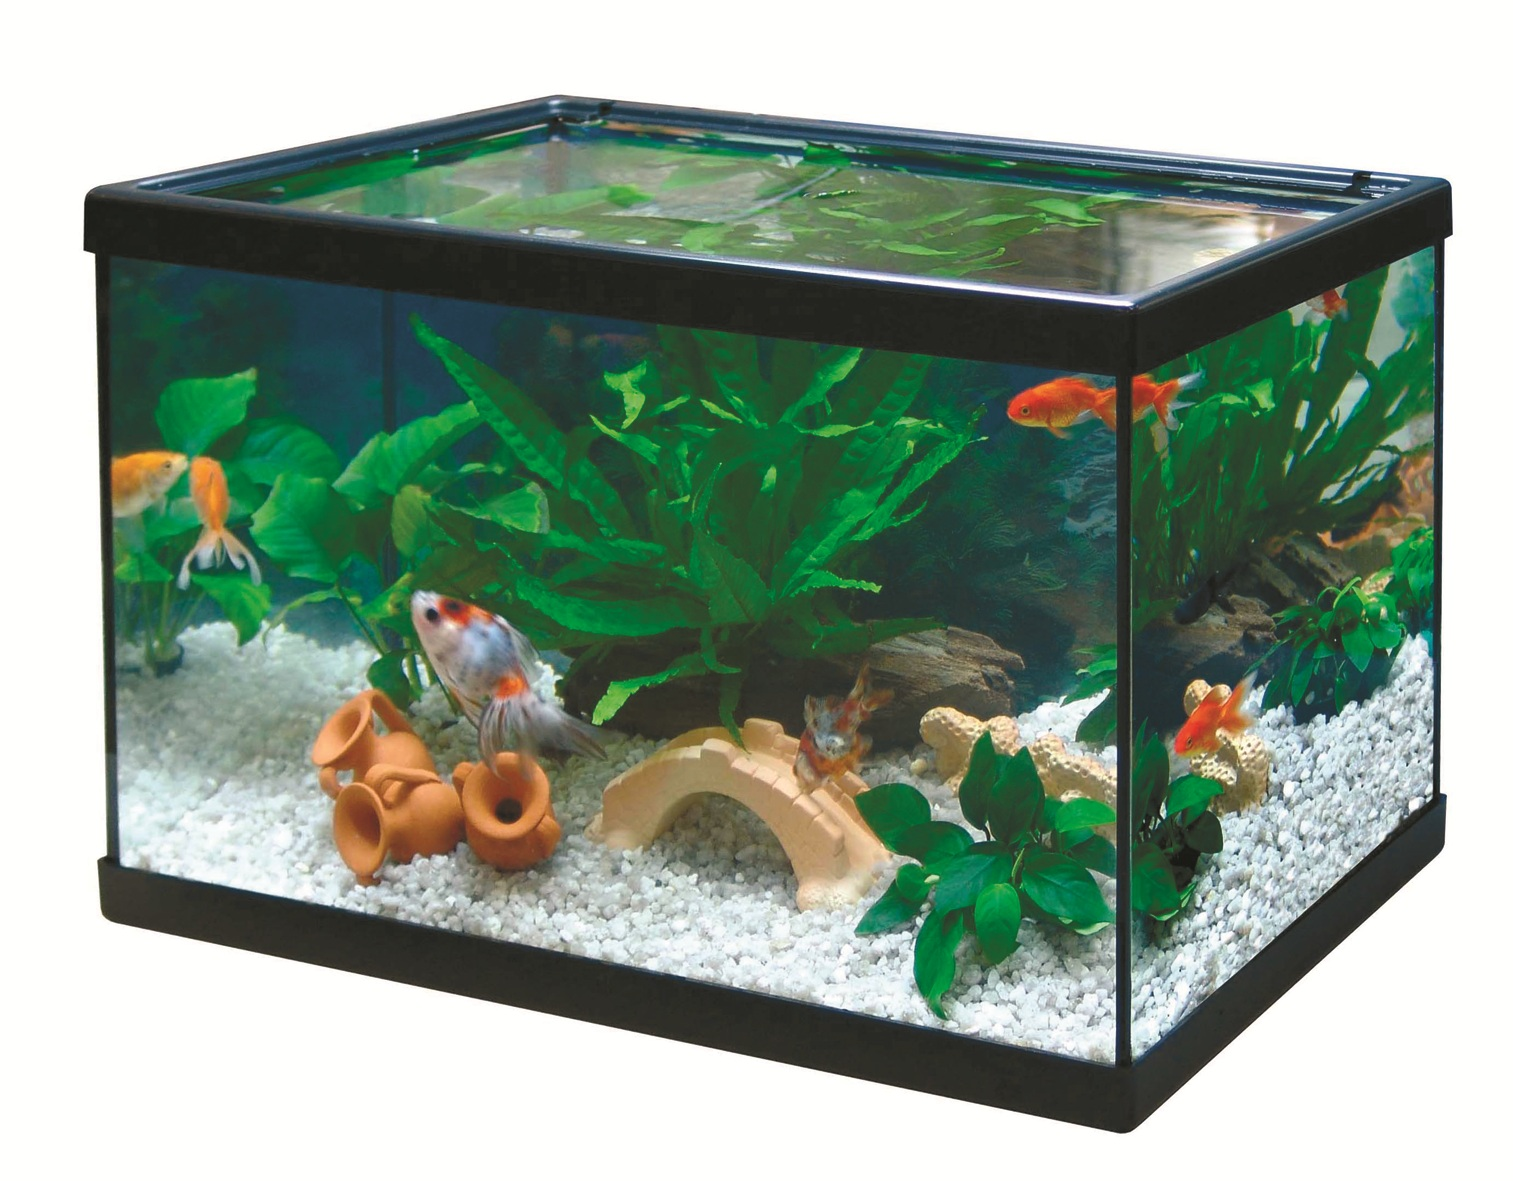
\includegraphics[width=1.7\textwidth]{./imagenes/acuario.jpg}
	\end{figure}	  	  	
  \end{minipage}
\end{minipage}
\end{frame}

\begin{frame}{\LARGE{\textbf{Nemo vale u\$d 300 ...}}}
	\begin{figure}[H]
		{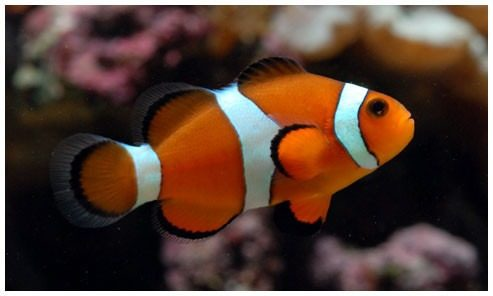
\includegraphics[width=1\textwidth]{./imagenes/nemo.jpg}}
	\end{figure}	  	  	
\end{frame}


\section[Problema]{Planteo del problema a resolver}

\begin{frame}{\textbf{\LARGE{Planteo del problema a resolver}}}
\fontsize{18pt}{18}\selectfont
	\begin{itemize}
		\item {¿Qué hace falta medir?}
		\vspace{20px}
		\item ¿Qué hace falta controlar?
		\vspace{20px}
		\item ¿Sobre qué hace falta alertar?
		\vspace{10px}
	\end{itemize}
\end{frame}

\begin{frame}{\textbf{\LARGE{¿Qué hace falta medir?}}}
\fontsize{18pt}{18}\selectfont
\begin{minipage}[c]{1.0\linewidth}
      \centering
      \begin{itemize}
		\item Nivel de agua		
		\vspace{20px}
		\item Temperatura
		\vspace{20px}      	
      	\item pH
		\vspace{20px}
	\end{itemize}
\end{minipage}
\end{frame}
	

\begin{frame}{\textbf{\LARGE{¿Qué hace falta controlar?}}}
\fontsize{18pt}{18}\selectfont
\begin{minipage}[c]{1.0\linewidth}
    \centering
	\begin{itemize}
		\vspace{-20px}
		\item Inyección de $O_2$/$CO_2$
		\vspace{15px}
		\item Iluminación
		\vspace{15px}
		\item Bombas de agua entrada/salida
		\vspace{15px}
		\item Calefactor
	\end{itemize}
\end{minipage}
\end{frame}

\begin{frame}{\textbf{\LARGE{¿Sobre qué hace falta alertar?}}}
\fontsize{18pt}{18}\selectfont
\begin{itemize}
	\item Parámetros fuera de rango
	\vspace{20px}
	\item 2 alarmas por sensor
	\vspace{20px}
	\item Indicación visual: Rojo/Verde
\end{itemize}	
\end{frame}


\section{Implementación}

\begin{frame}{\textbf{\LARGE{CIAA-NXP}}}
	\vspace{-.7cm}
	\begin{figure}[H]
		{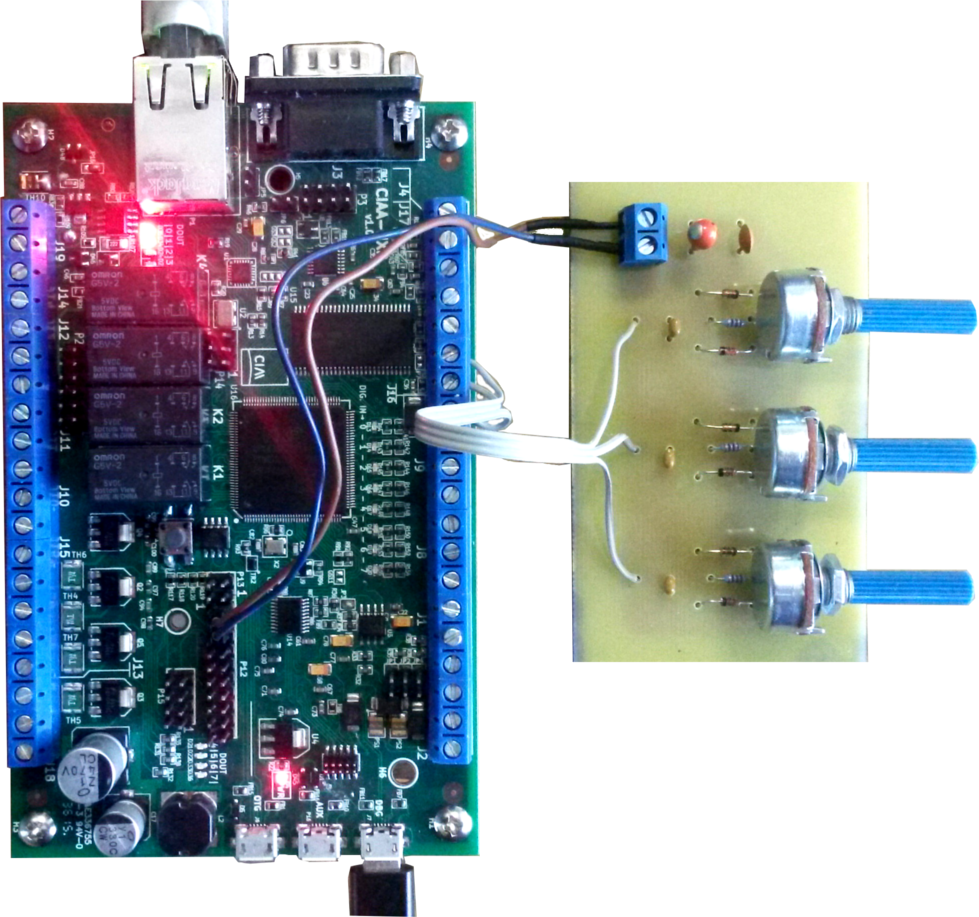
\includegraphics[width=.7\textwidth]{./imagenes/ciaa.png}}
	\end{figure}	
\end{frame}

\begin{frame}{\textbf{\LARGE{Arquitectura del Software}}}
	\begin{figure}[H]
		{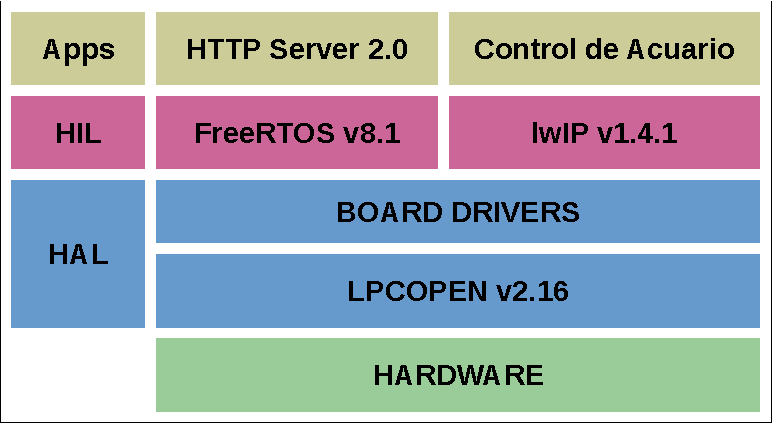
\includegraphics[width=1\textwidth]{./imagenes/bloques.pdf}}
	\end{figure}	  	  	
\end{frame}

\begin{frame}{\textbf{\LARGE{Interfaz Web}}}
	\Wider{
	\begin{figure}[H]
		{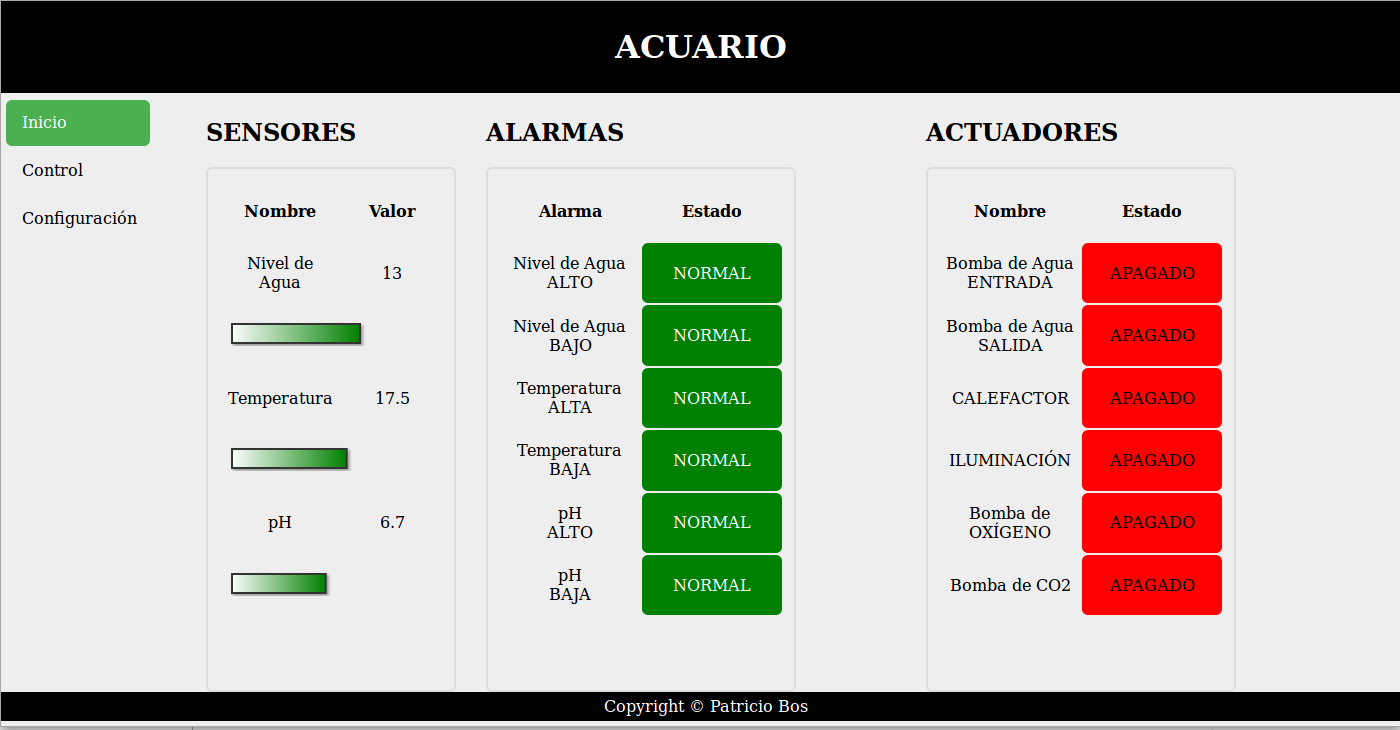
\includegraphics[width=1\textwidth]{./imagenes/interfaz_home_normal.png}}
	\end{figure}	  	  	
	}
\end{frame}


\begin{frame}{\textbf{\LARGE{Interfaz Web}}}
		\Wider{
	\begin{figure}[H]
		{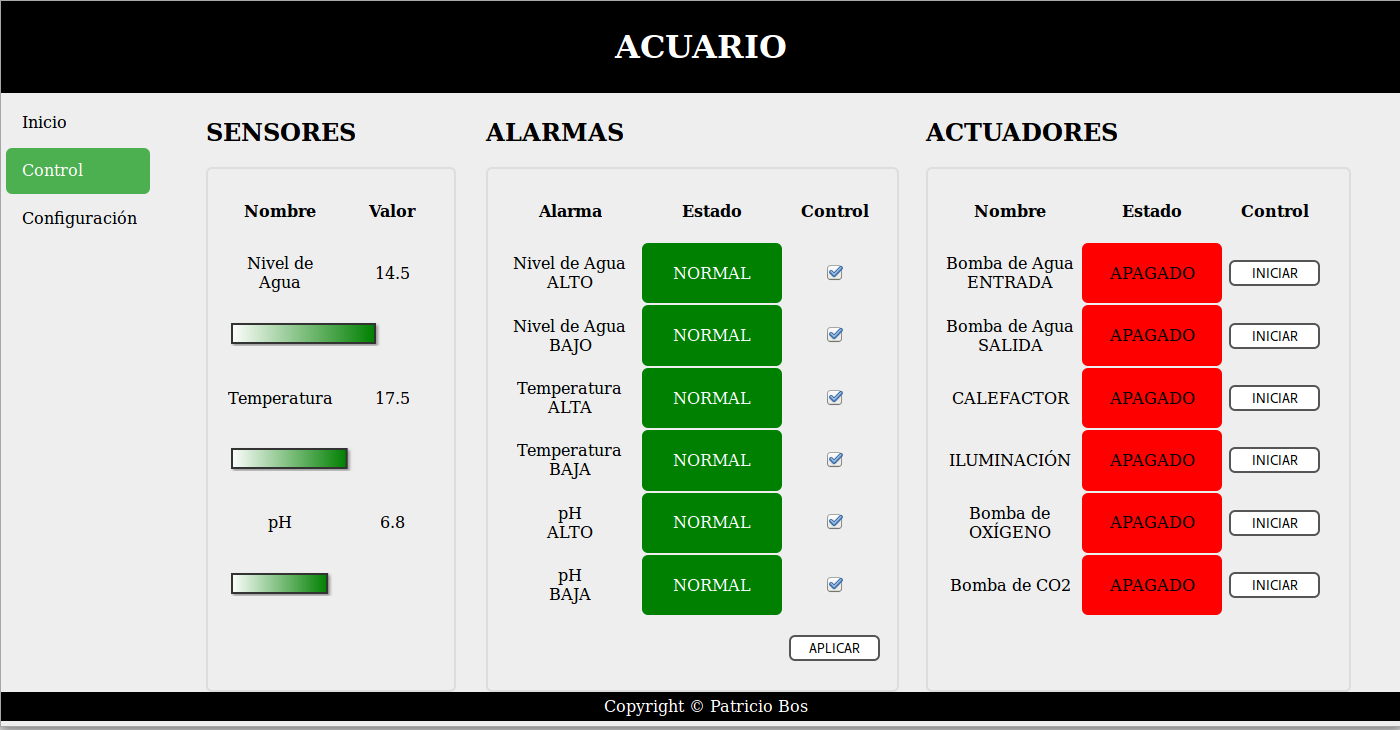
\includegraphics[width=1\textwidth]{./imagenes/interfaz_control_normal.png}}
	\end{figure}	
	}  	  	
\end{frame}



\begin{frame}{\textbf{\LARGE{Interfaz Web}}}
	\Wider{	
	\begin{figure}[H]
		{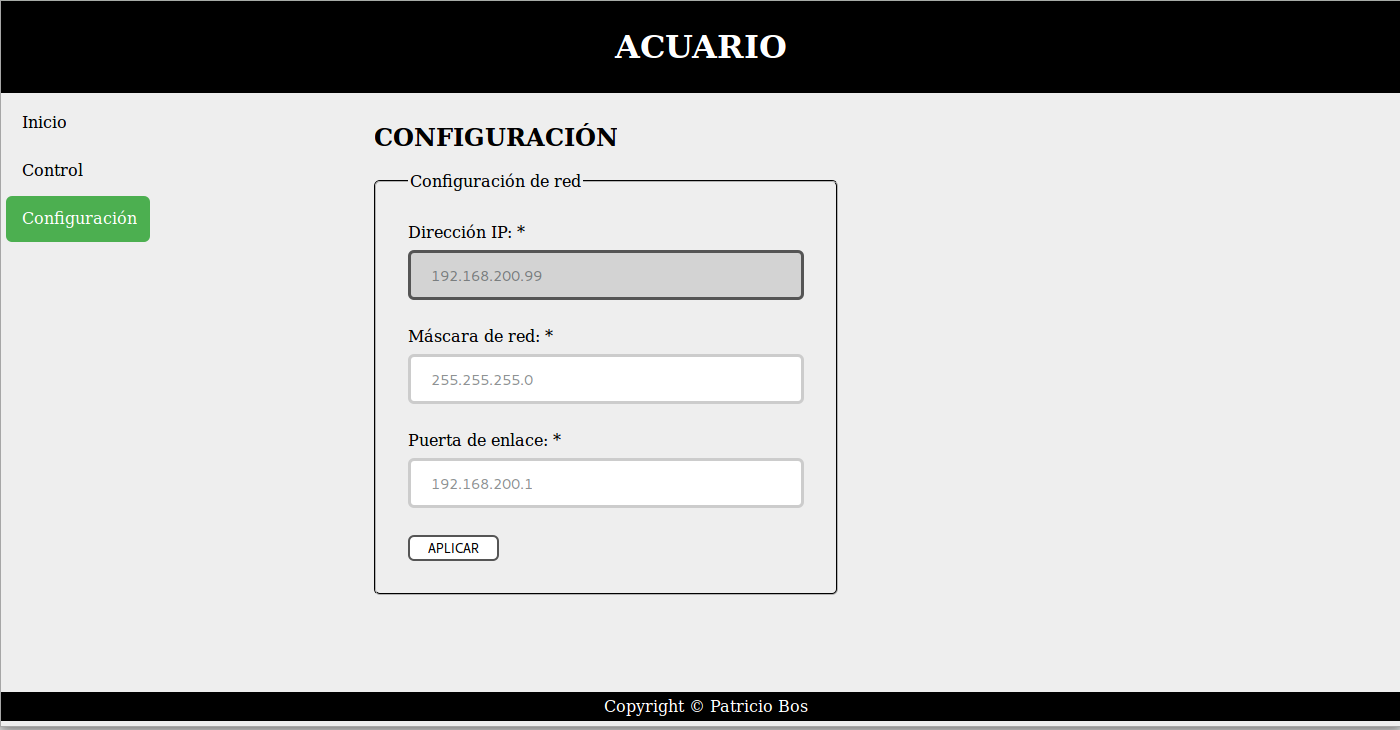
\includegraphics[width=1\textwidth]{./imagenes/interfaz_config}}
	\end{figure}	  	  	
	}
\end{frame}

\begin{frame}{\textbf{\LARGE{Tecnologías utilizadas}}}
\fontsize{18pt}{18}\selectfont
	\begin{itemize}
		\item Webserver HTTP 2.0
		\vspace{10px}
		\item JavaScript
		\vspace{10px}		
		\item Server Side Includes (SSI)
		\vspace{10px}
		\item Asynchronous JavaScript and XML (AJAX)
		\vspace{10px}
		\item Common Gateway Interface (CGI)
	\end{itemize}
\end{frame}

\section{Ensayos y validación}

\begin{frame}{\textbf{\LARGE{Ensayos - Tabla de decisión}}}
	\vspace{-10px}
	\Wider{	
	\begin{figure}[H]
		{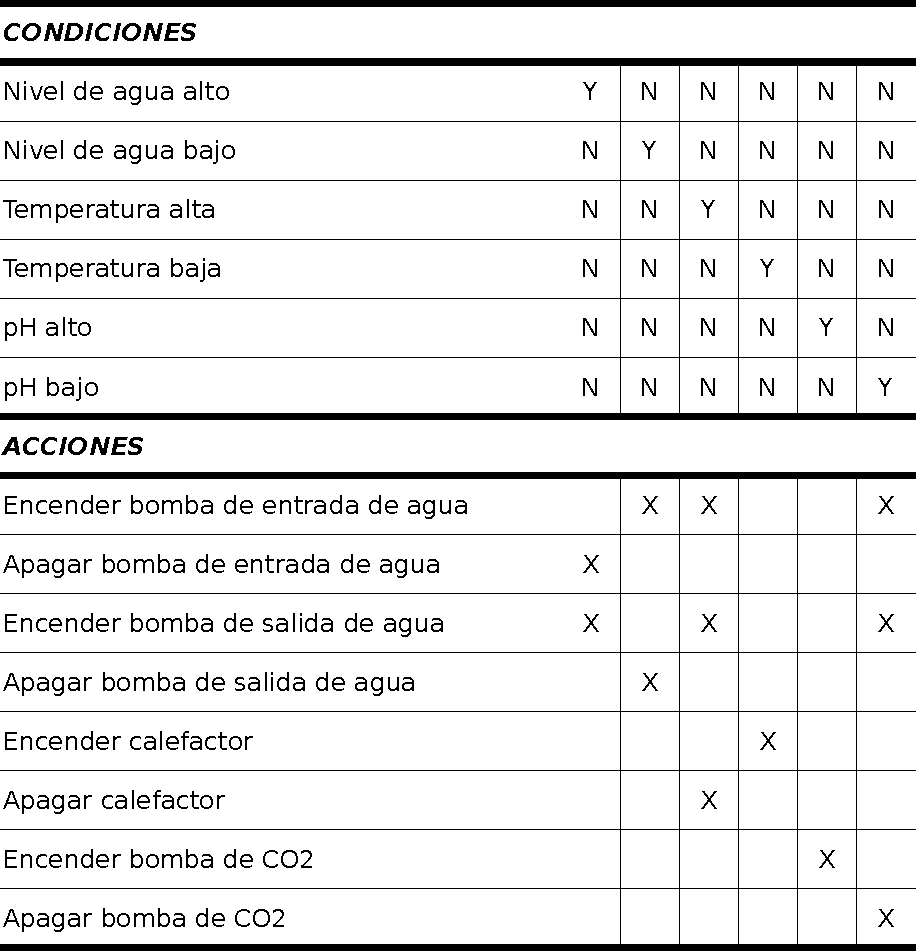
\includegraphics[height=.8\textheight]{./imagenes/tabla1alarma}}
	\end{figure}	  	  	
	}
\end{frame}

\begin{frame}{\textbf{\LARGE{Ensayos - Nivel de agua}}}
	\Wider{	
	\begin{figure}[H]
		{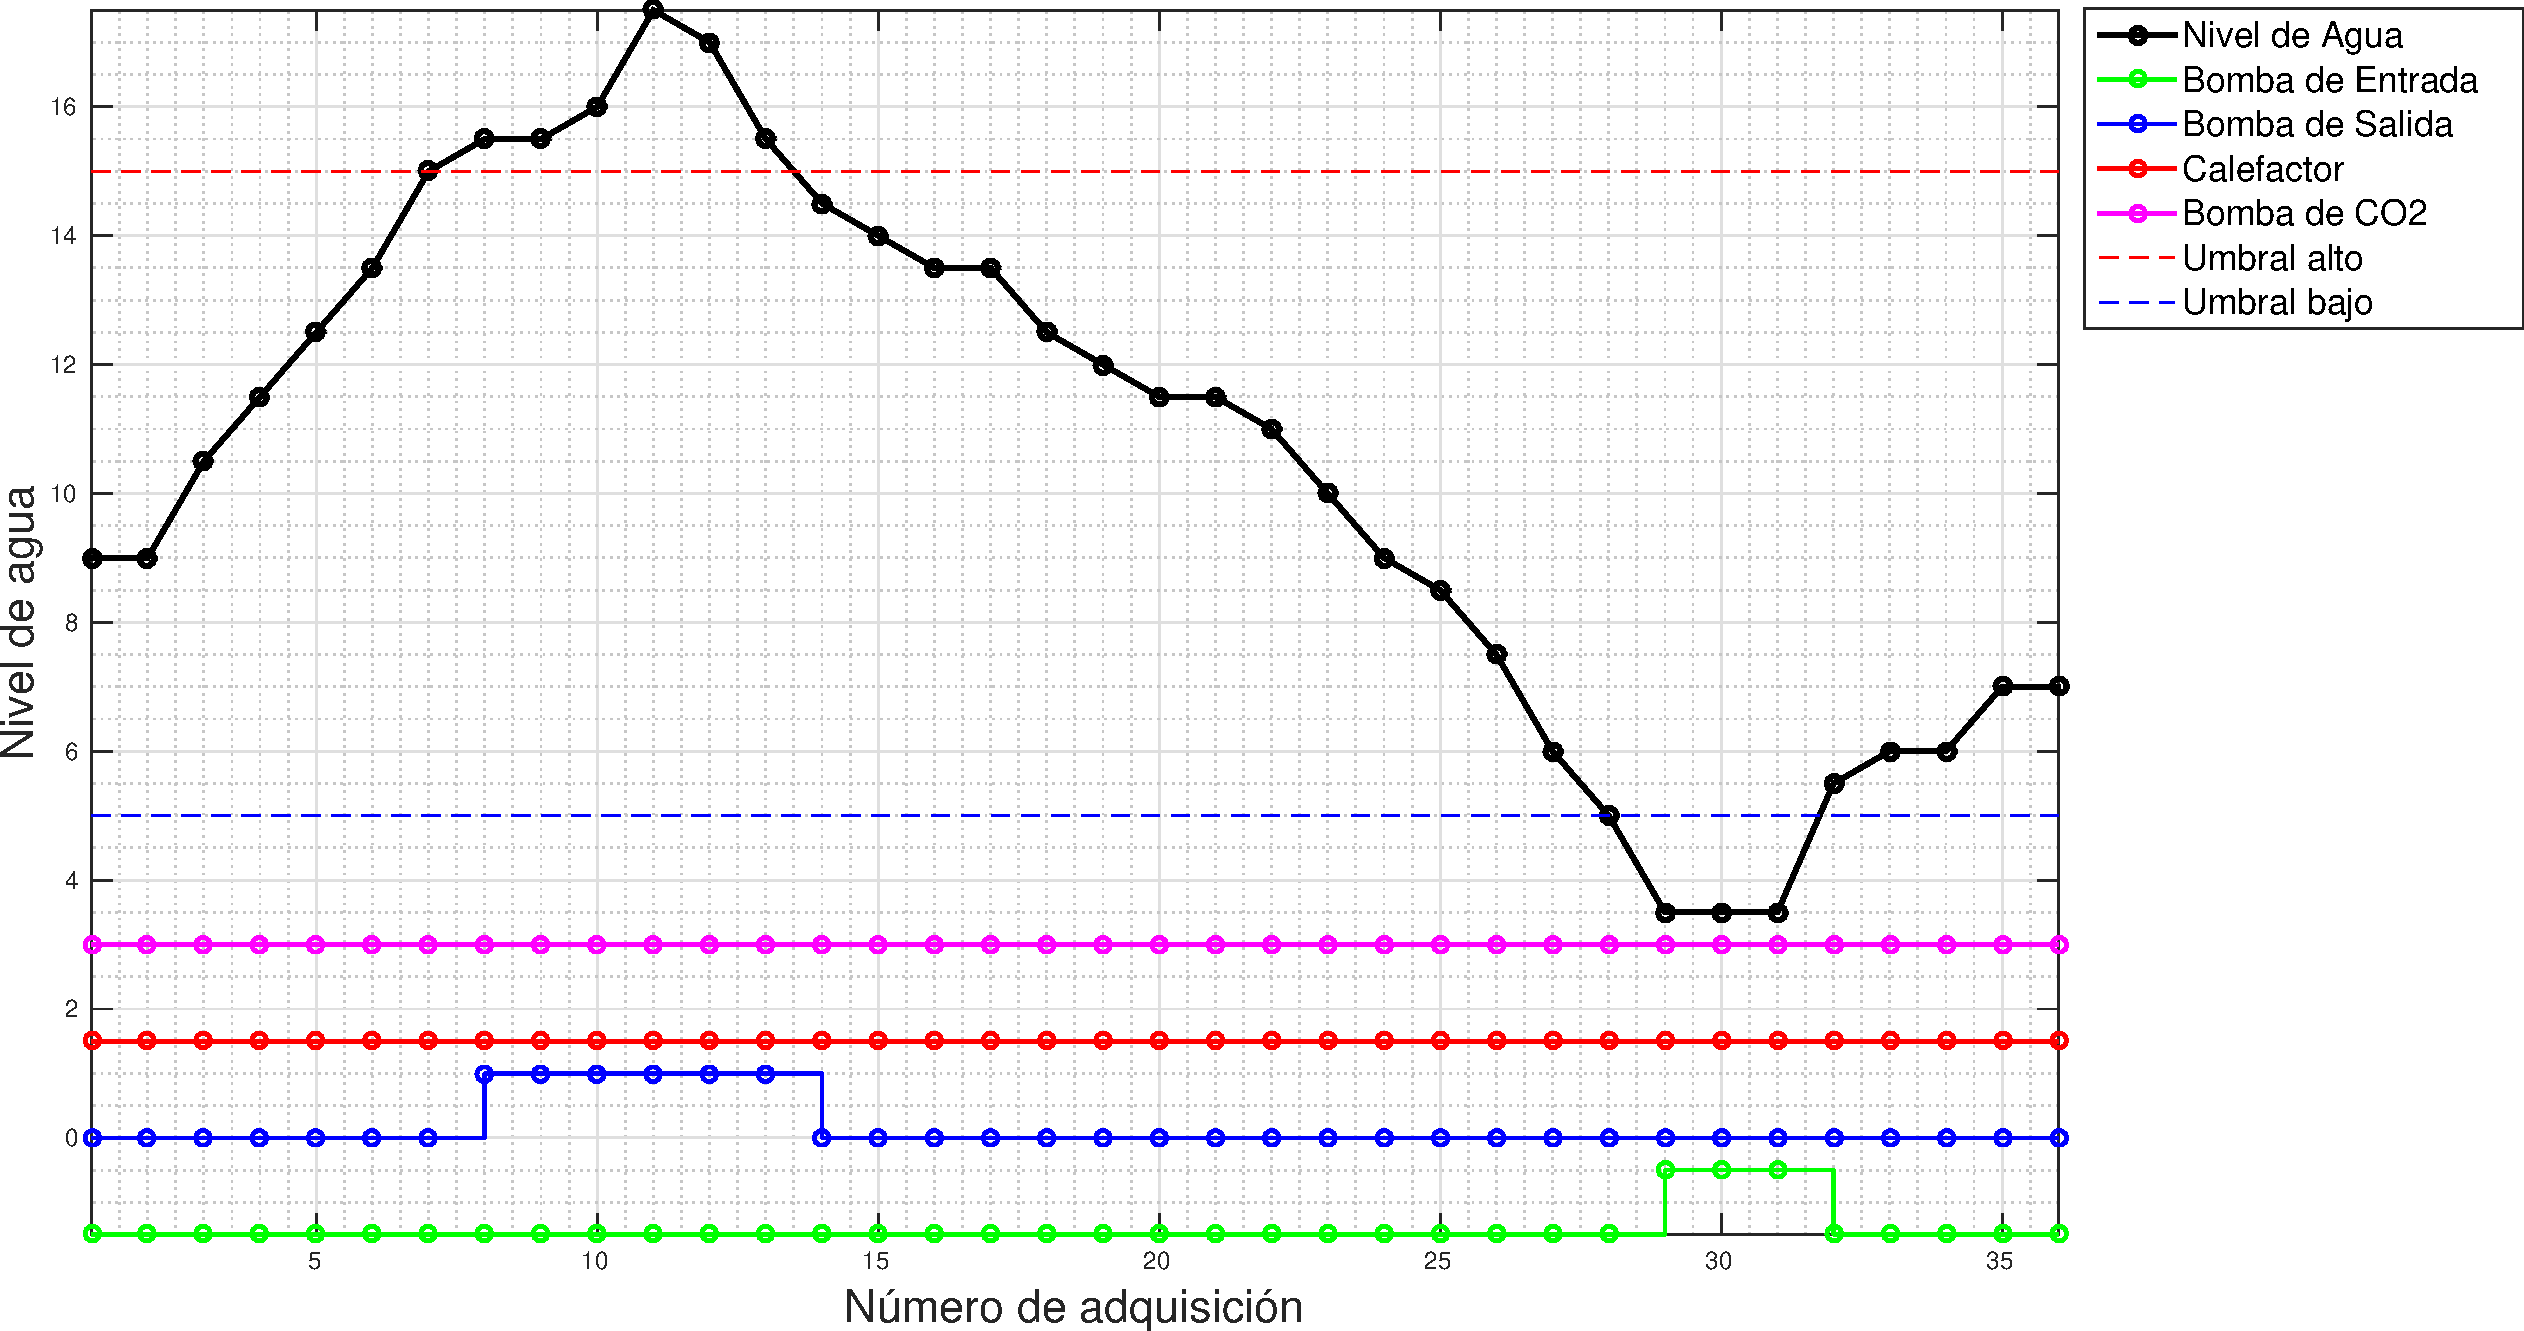
\includegraphics[width=1\textwidth]{./imagenes/plot1Water}}
	\end{figure}	  	  	
	}
\end{frame}

\begin{frame}{\textbf{\LARGE{Ensayos - Temperatura}}}
	\Wider{	
	\begin{figure}[H]
		{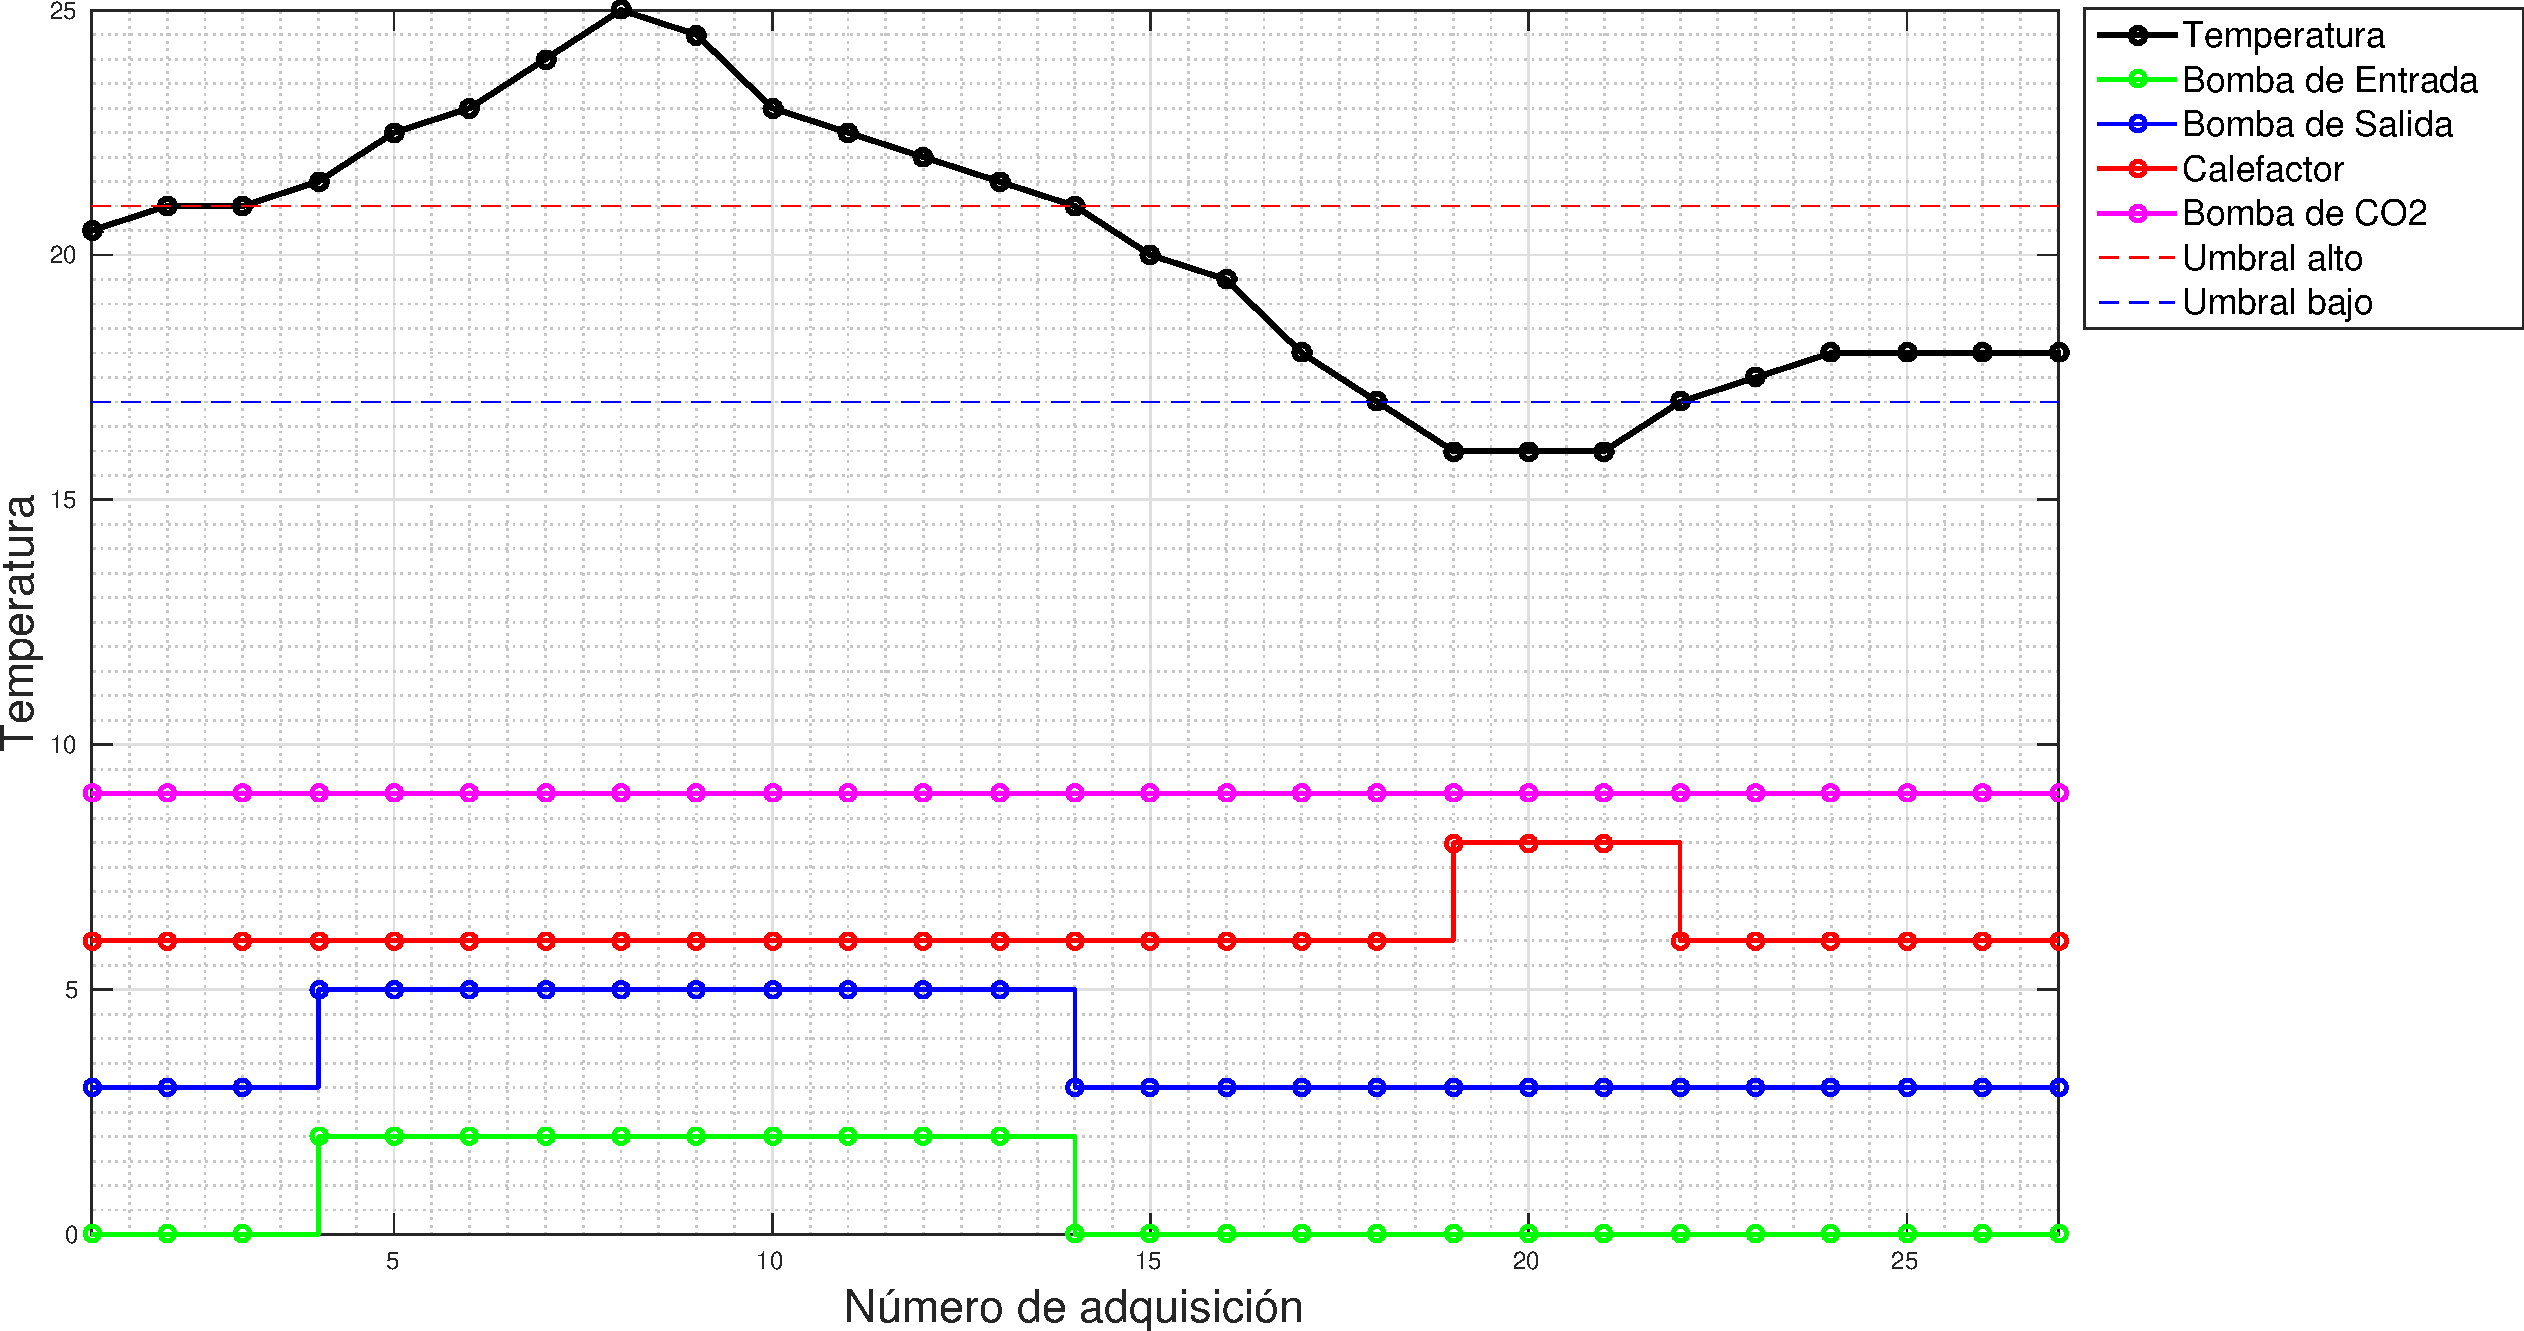
\includegraphics[width=1\textwidth]{./imagenes/plot1Temp}}
	\end{figure}	  	  	
	}
\end{frame}

\begin{frame}{\textbf{\LARGE{Ensayos - pH}}}
	\Wider{	
	\begin{figure}[H]
		{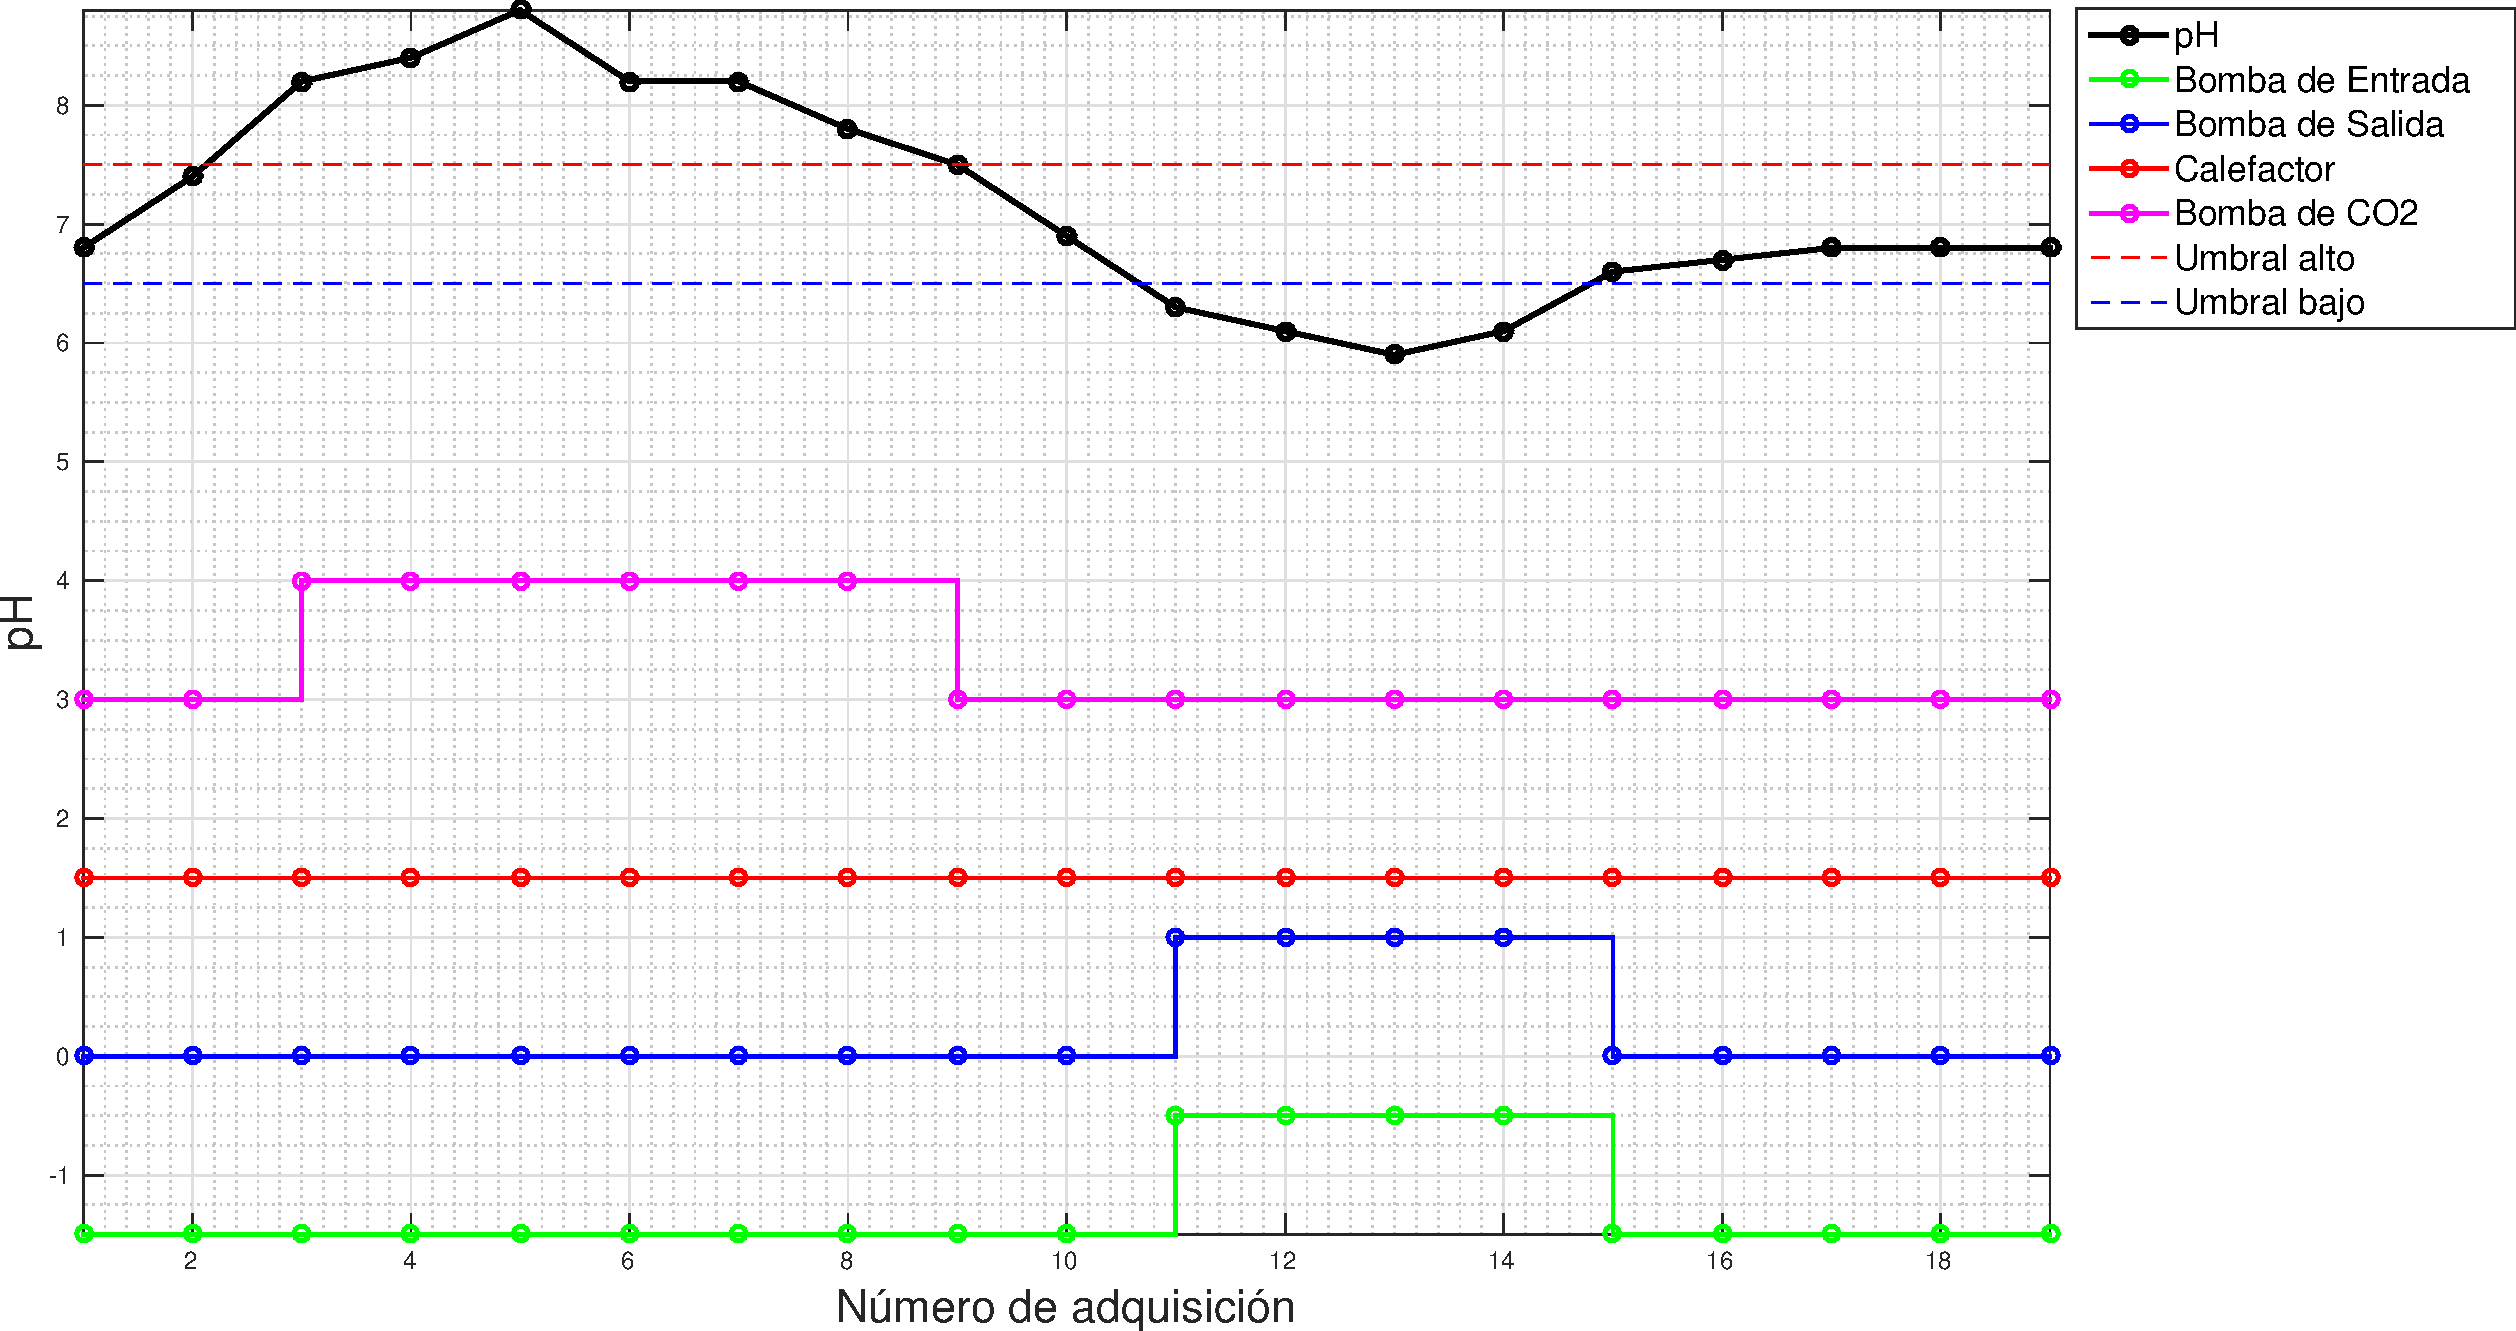
\includegraphics[width=1\textwidth]{./imagenes/plot1pH}}
	\end{figure}	  	  	
	}
\end{frame}

\section{Demostración}


\section{Conclusiones}

\begin{frame}{\textbf{\LARGE{Conclusiones}}}
	\fontsize{16pt}{16}\selectfont
	\begin{itemize}
		\item Se desarrolló un firmware que cumple con los criterios de aceptación.
		\vspace{10px}
		\item Se aplicaron los conocimientos adquiridos en la carrera para obtener un sistema embebido sobre la CIAA-NXP.
		\vspace{10px}
		\item Se logró un código modular con posibilidades de aplicación a otros proyectos.
	\end{itemize}
\end{frame}

\begin{frame}{\textbf{\LARGE{Trabajo Futuro}}}
	\fontsize{16pt}{16}\selectfont
	\begin{itemize}
		\item Migrar el RTOS a freeOSEK.
		\vspace{15px}
		\item Mejorar el soporte para cambios en el dominio de aplicación.
		\vspace{15px}
		\item Optimizar el acceso desde dispositivos móbiles.
	\end{itemize}
\end{frame}

\begin{frame}[plain,noframenumbering]
	\begin{center}
\vspace{5px}	
	\large\textbf{Carrera de Especialización en Sistemas Embebidos}\\
	\vspace{10px}
	\Large\textbf{Presentación de Trabajo Final}\\
	\vspace{5px}
	\hfill
	    \begin{beamercolorbox}[center,dp=2ex,ht=.25\textheight, wd=1\paperwidth]{bgcolor}
	        \huge\textbf{Control de acuario con la CIAA}\\
	    		\vspace{5px}
			\Large\textbf{Ing. Patricio Bos}\\
			%\texttt{pbos@fi.uba.ar}
	    \end{beamercolorbox}
	\hfill\hfill
	\\
	\vspace{-5px}
	%\vfill
	\begin{minipage}[t]{0.4\textwidth}
		\begin{flushleft} \large
			\textbf{Director:}\\
			Ing. Juan Manuel Cruz\\
		\end{flushleft}
	\end{minipage}
	\begin{minipage}[t]{0.4\textwidth}
		\begin{flushright} \large
			\textbf{Jurados:} \\
			Ing. Ramiro Alonso \\
			Ing. Eric Pernia\\
			Ing. Pablo Ridolfi\\
		\end{flushright}
	\end{minipage}
	\vfill
	\begin{figure}[H]
		
\includegraphics[width=2cm]{./imagenes/logo_facu_circle}
	\end{figure}	
	\vspace{5px}
	\end{center}
\end{frame}



\end{document}
